\documentclass[11pt]{article} 
\usepackage[utf8]{inputenc} 
\usepackage{geometry} 
\geometry{a4paper} 
\usepackage{graphicx}





\title{Big Data Analytics Project : Dataset Adult from UCI }
\author{Mohammed Meftah, Raunaq Paul and Binxiang Xiang}
\date{$16^{th}$ January 2017}

\begin{document}
\maketitle
\tableofcontents

\newpage
\section{Introduction}
For this project, we have decided to work on the dataset Adult from UCI. This is a classification dataset with two classes, as we have to understand and predict whether a person earns less or more than 50k dollars a year, according to the provided features. Section 2 describes in details the used dataset Adult. Section 3 highlights how we first processed data. Section 4 shows some statistical analysis on the dataset. Section 5 presents the methodology and the performances of different algorithms (list of tried algo to add) on the prediction of our target variable. 

\section{Dataset description}
The raw dataset has 48842 rows and 15 columns including the target variable. This data is originally from the american census bureau and shoulb be representative of the american population. This dataset is mixing continuous variables and discrete variables as follows : 

\begin{description}\itemsep0.5pt
\item[age] : continuous, age of the individual.
\item[fnlwgt] : continuous, the number of people the observation should represent, not useful for us.
\item[workclass] : discrete, 8 categories representing the type of the employer of the individual ( Private, Federal-gov, Never-worked ...).
\item[education] : discrete, 16 categories representing the highest level of education achieved by the individual (Bachelors, Masters, Doctorate, Highschool grad ... ).
\item[educationnum] : continuous, number of years of education.
\item[mstatus] : discrete, 7 categories representing the marital status of the individual(Divorced, Never-married, Separated ... ).
\item[occupation] : discrete, 14 categories representing the occupation of the individual (Tech-support, Sales, Exec-managerial, Other-service ...).
\item[relationship] : discrete, 6 categories representing the relationship of the individual, we don't know with who so this variable is not very clear (Wife, Husband,Own-child ...).
\item[race] : discrete, 5 categories representing the race of the individual (White, Asian-Pac-Islander, Black, Amer-Indian-Eskimo and Other).
\item[sex] : discrete, sex of the individual (Female or Male).
\item[capitalgain] : continuous, represents the recorded capital gains.
\item[capitalloss] : continuous, represents the recorded capital losses.
\item[hoursperweek] : continuous, represents the number of hours worked per week.
\item[nativecountry] : discrete, 41 categories representing the country of origin of the individual.
\item[target] : discrete, variable to predict, 2 classes ($<= 50k\$$ or $>50k\$$).
\end{description}
For the next sections, these names will be used to refer to the corresponding variable.
\section{Data processing}
In this section, we explain the different steps of processing we did on our raw dataset.
\subsection{Basic processing : }
We did perform some basic processing as a first step : 
\begin{itemize}
\item Remove the variable \emph{fnlwgt}, as it is not an information on the individual.
\item Remove the variable \emph{education}, as it contains the same information as the variable \emph{educationnum} and we would prefer to work with a continuous variable.
\item Transform the target variable into binary values,  0 if $<=50k\$$ 1 if $>50k\$$.
\item Remove rows with missing values, indeed variables \emph{workclass}, \emph{occupation} and \emph{nativecountry} don't always have values. It represents 3620 rows.
\item Scale continuous variables : \emph{educationnum,capitalgain,capitalloss and hoursperweek}
\end{itemize}
After these steps, the new dataset has 45222 rows. And 24.8\% of the observations are in the class 1 and 75.2\% are in the class 0.
\subsection{Advanced processing :}
As the discrete variable \emph{nativecountry} contains 41 categories where the main one (United States) represents 91.3\% of the total, we have decided to group countries together into bigger categories. We don't change United-States, Canada, Japan, China, India , Iran and Mexico. The changes are the following :

\begin{center}

\begin{tabular}{|c|c|}
\hline
New value & Old values concerned \\
\hline
WEurope & England, France, Germany, Holand-Netherlands,\\
& Ireland, Italy, Portugal, Scotland\\
\hline
EEurope & Greece, Hungary, South, Yugoslavia\\
\hline
SEAsia & Cambodia, Laos, Philippines, Thailand, Vietnam\\
\hline
 LatAmerica & Columbia, Cuba, Dominican-Republic, Ecuador, El-Salvador, \\
&Guatemala, Haiti, Honduras, Jamaica, Nicaragua, \\
&Outlying-US(Guam-USVI-etc), Peru, Puerto-Rico, Trinadad\&Tobago \\
\hline
China & HongKong, Taiwan \\
\hline
\end{tabular}
\end{center}
After the transformation, our \emph{nativecountry} variable has now 11 different values against 41 before. Of course, we lost some information but it shoud not be so significant as we regroup countries from same area and with similar economic situation.



\section{Analysis}
After the processing part, we can start to look at data and make some analysis by variable and with by class. We separated the study whether the variables are nummeric or categorical.

\subsection{Numerical features}
We first study the correlation of numerical variables with the target. We thus made the following corrplot :

\begin{figure}[!h]
	\centering
	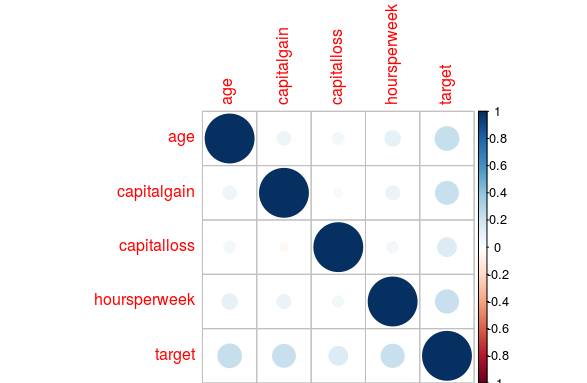
\includegraphics[width=.6\textwidth]{images/plot_corr.png}
\end{figure}
It shows that all the numerical variables are correlated positively with the target. However the correlation values remains low with the best score for (age, target) around 0.3. So for a first model, maybe it is not of paramount importance to include such variables.

\subsection{Categorical features}
We cannot define a correlation properly with categorical variables. We choose to look at the distribution of the target within the categorical variables and test their independance ($\chi$-squared test) with the target in order to have an idea of each possible contribution.

\begin{center}
\begin{tabular}{|c|c|c|}
Feature & $\chi$-square & $p$-value \\
\hline
race & 452.3 & $<$2.2e-16\\
workclass & 1207.3 & $<$2.2e-16\\
mstatus & 9109.2 & $<$2.2e-16\\
sex & 2104.1 & $<$2.2e-16\\
nativecountry & 379.36 & $<$2.2e-16 \\
education & 6000 & $<$2e-16
\end{tabular}
\end{center}

The $\chi$-square test are very concluding so we are confident to reject the null hypothesis and consider that each of these categorical variables are non-independant with the target, it means that they are correlated. The very low p-values pinpoint also this high correlation. We should see some pattern by looking at the target distribution for each unique element of each feature.


\begin{figure}[!h]
	\centering
	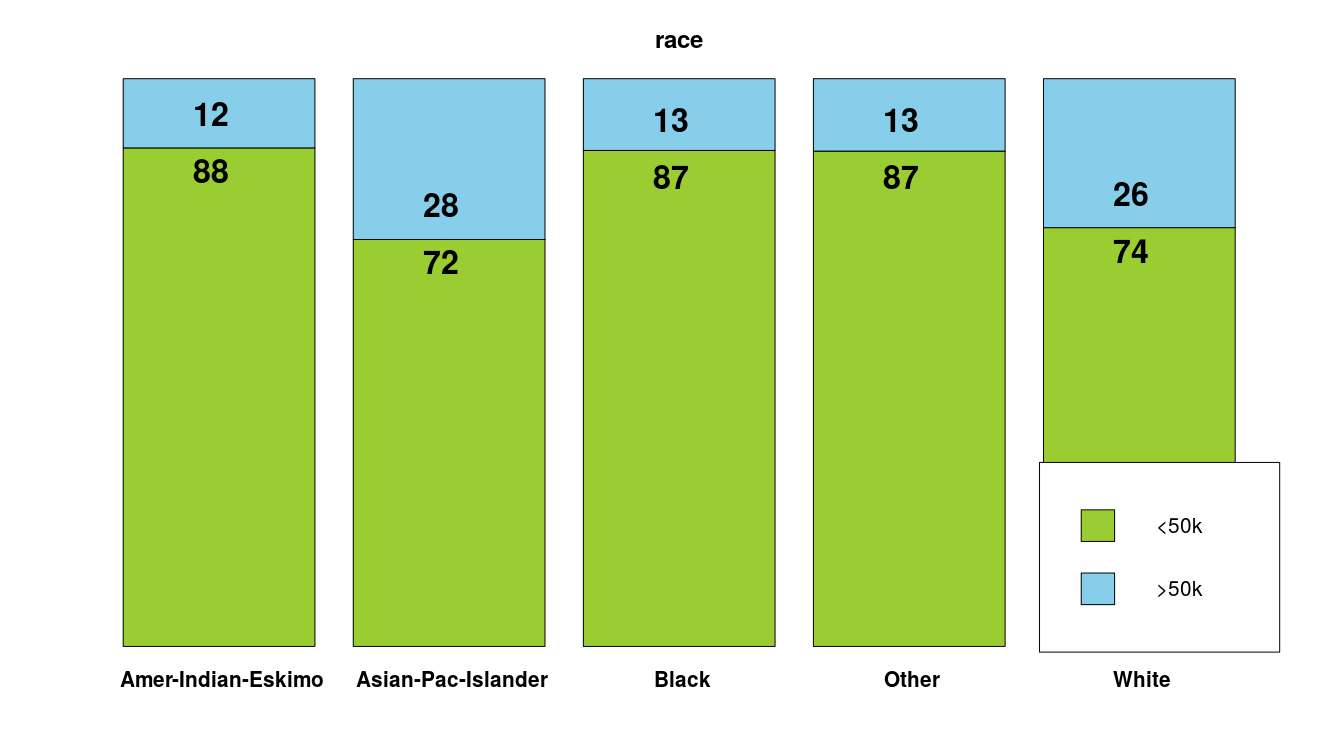
\includegraphics[width=.5\textwidth]{images/plot_race.png}%
	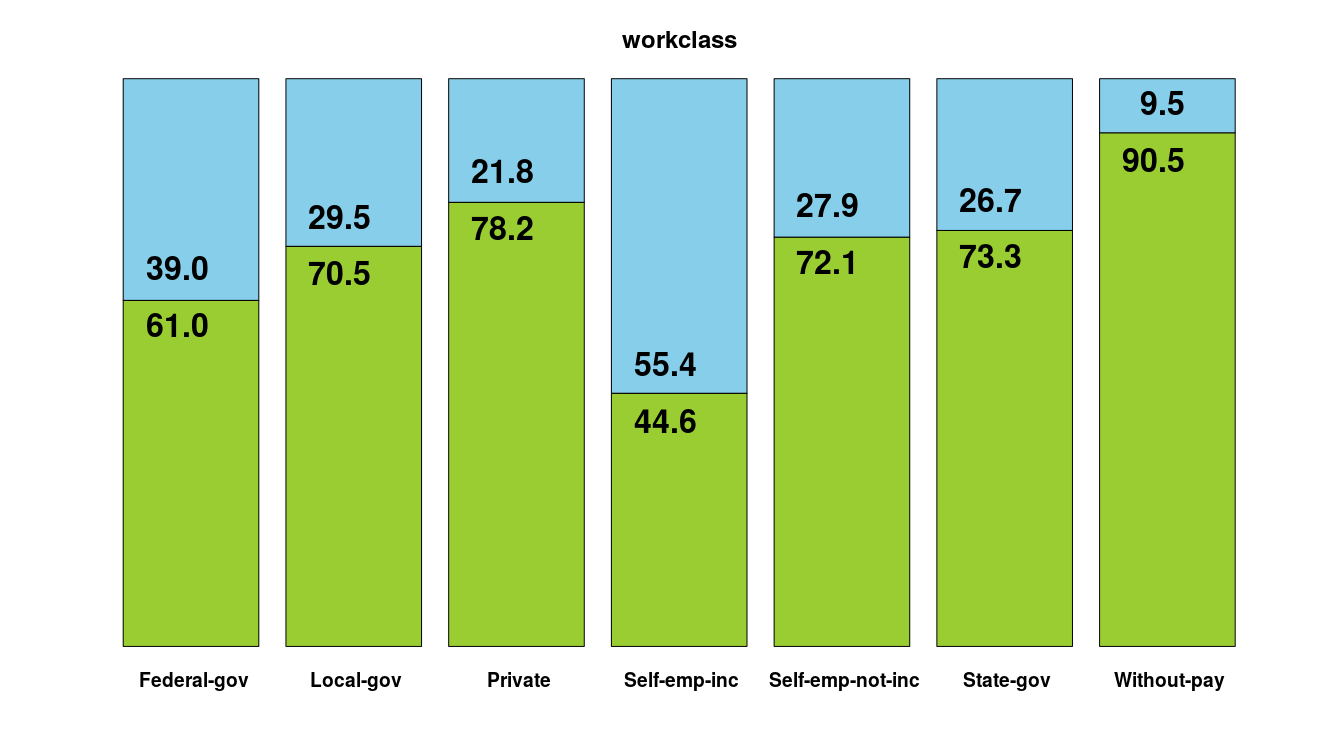
\includegraphics[width=.5\textwidth]{images/plot_workclass.png}
	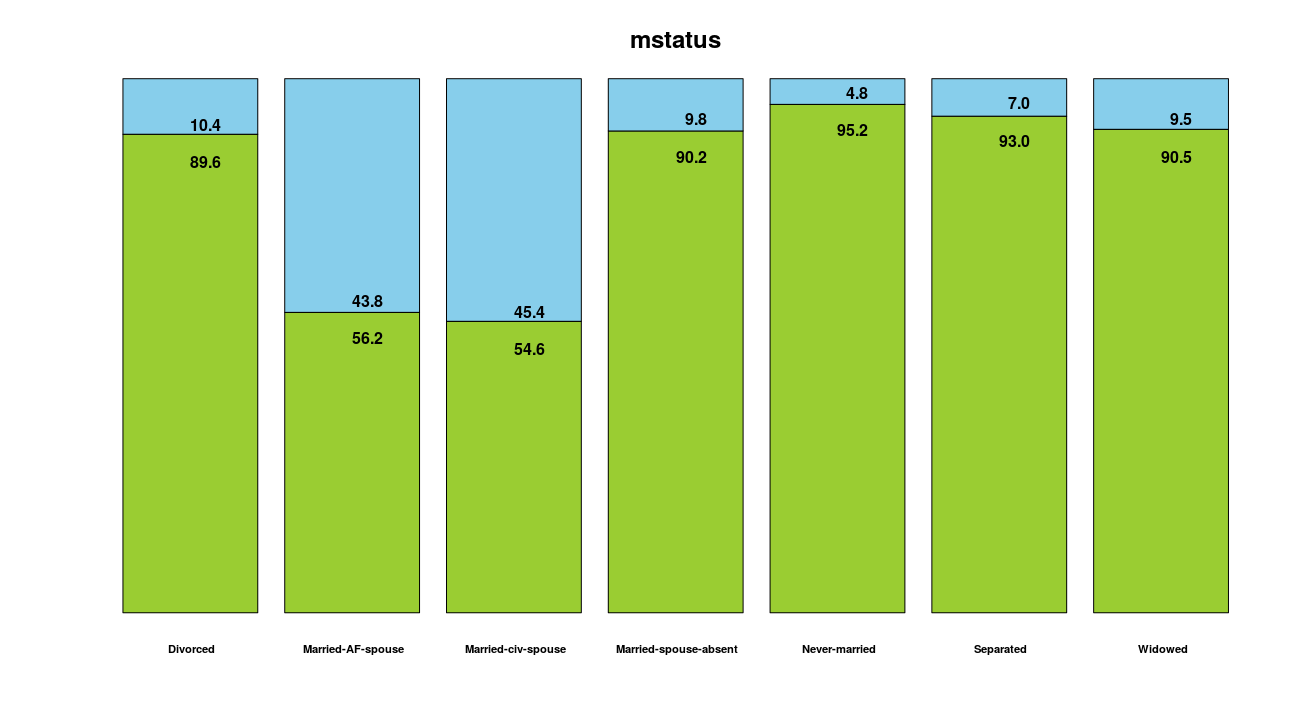
\includegraphics[width=.5\textwidth]{images/plot_mstatus.png}%
	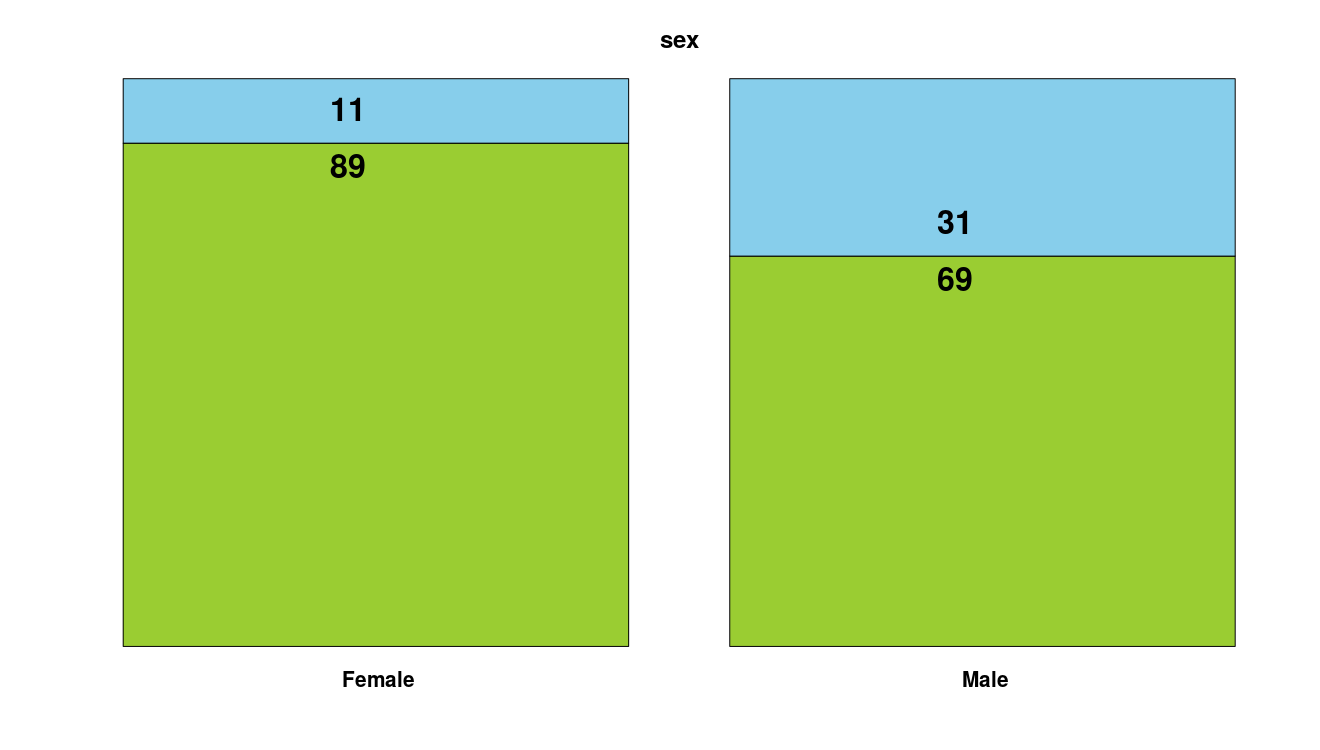
\includegraphics[width=.5\textwidth]{images/plot_sex.png}
	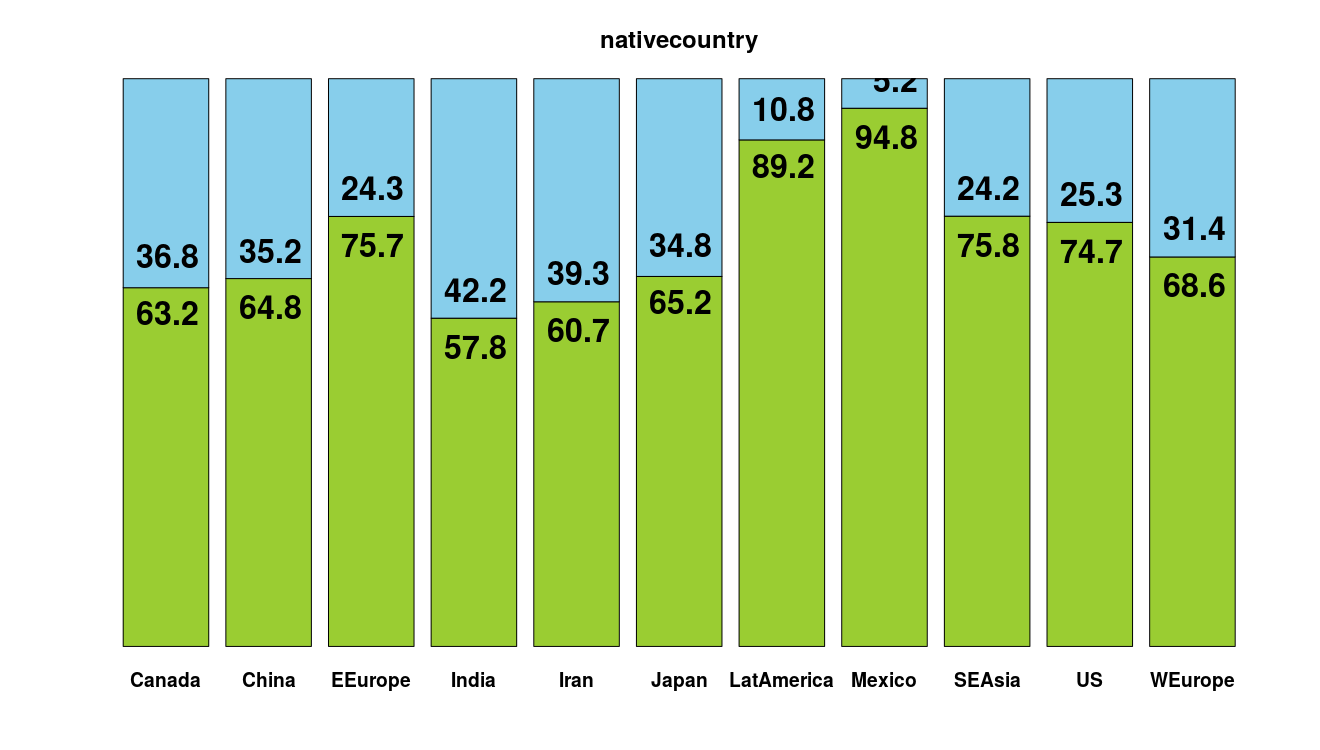
\includegraphics[width=.5\textwidth]{images/plot_nativecountry.png}%
	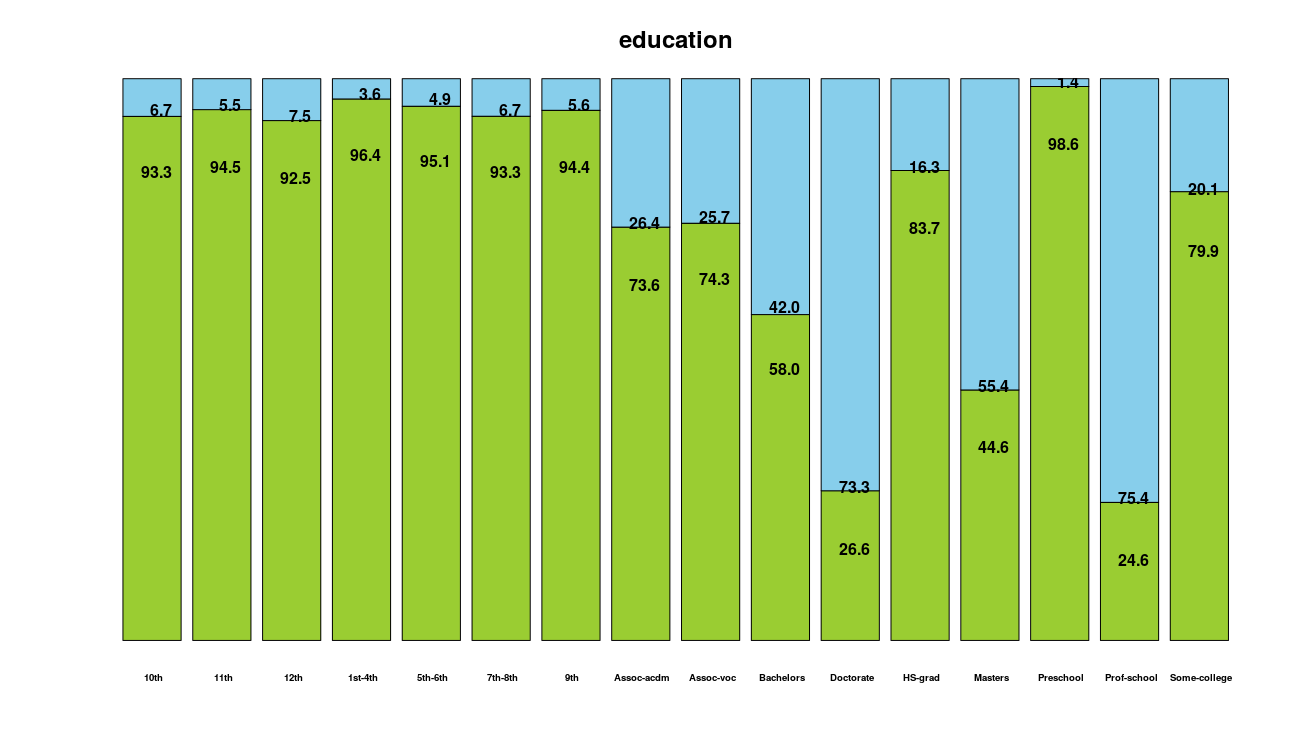
\includegraphics[width=.5\textwidth]{images/plot_education.png}
\end{figure}

As we clearly see, for altmost all this categorical features, the distribution of the target is not homogenous within the feature labels. It should enable us to make better predictions with these features as a basis.

\section{Methodology and results}
\section{Conclusion}







\end{document}
